\item Sean $\E$ la base canónica de $\R^3$ y $B=\{(1,1,0);(1,1,1);(0,1,1)\}$.
    \begin{enumerate}
        \item Hallar la matriz $P_{\E,B}$ de cambio de base de $B$ en $\E$.
            \begin{mdframed}[style=s]
                \begin{center}
                    $P_{\E,B}=\left([(1,1,0)]_\E\quad[(1,1,1)]_\E\quad[(0,1,1)]_\E\right)$\\
                    $P_{\E,B}=\begin{pmatrix}
                        1&1&0\\1&1&1\\0&1&1
                    \end{pmatrix}$
                \end{center}
                En la Figura 1 se muestra como $[g]_B=\begin{pmatrix}
                    1&1&0
                \end{pmatrix}^T$, es escrito en términos de la base canónica.($[g]_\E=P_{\E,B}\cdot[g]_B=\begin{pmatrix}
                    2&2&1
                \end{pmatrix}^T$)
                \begin{center}
                    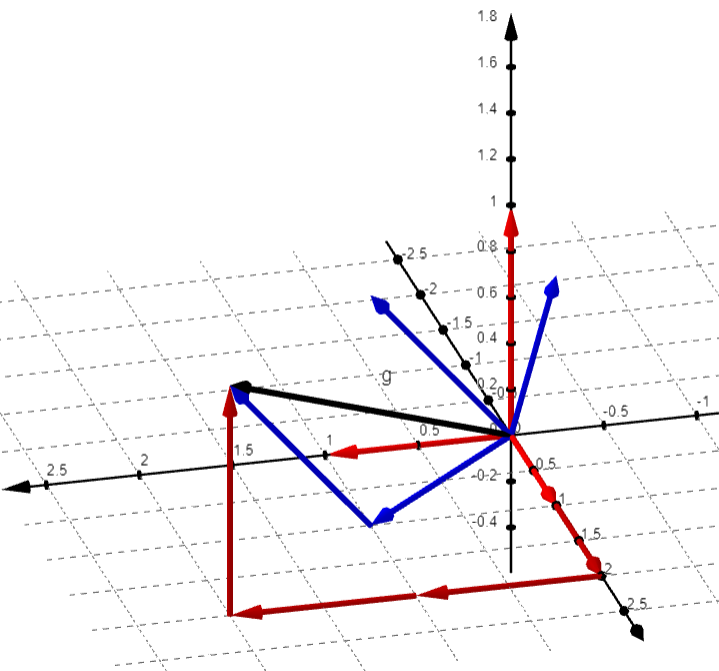
\includegraphics[width=0.4\textwidth]{img/Ej2a.png}\\
                    Figura 1. Vector g representado en dos bases diferentes.
                \end{center}
            \end{mdframed}
        \item Hallar la matriz $P_{B,\E}$ de cambio de base de $\E$ en $B$.
            \begin{mdframed}[style=s]
                \begin{center}
                    $P_{B,\E}=\left([(1,0,0)]_B\quad[(0,0,0)]_B\quad[(0,0,1)]_B\right)$\\
                    $P_{B,\E}=\begin{pmatrix}
                        0&1&-1\\1&-1&1\\-1&1&0
                    \end{pmatrix}$
                \end{center}
            \end{mdframed}
        \item Comprobar que la matriz hallada en el ítem $a)$ es la inversa de la del ítem $b)$.
            \begin{mdframed}[style=s]
                Para que sean inversas, su producto tiene que dar como resultado la matriz identidad:
                \begin{center}
                    $\begin{pmatrix}
                        1&1&0\\1&1&1\\0&1&1
                    \end{pmatrix}\cdot\begin{pmatrix}
                        0&1&-1\\1&-1&1\\-1&1&0
                    \end{pmatrix}=\begin{pmatrix}
                        1&0&0\\0&1&0\\0&0&1
                    \end{pmatrix}$
                \end{center}
            \end{mdframed}
        \item Comprobar que $P_{B,\E}[(1,2,0)]_\E=[(1,2,0)]_B$.
            \begin{mdframed}[style=s]
                Una forma sería:
                \begin{align*}
                    P_{B,\E}[(1,2,0)]_\E&=[(1,2,0)]_B\\
                    P_{B,\E}P_{\E,B}[(1,2,0)]_B&=[(1,2,0)]_B\\
                    I[(1,2,0)]_B&=[(1,2,0)]_B\\
                    [(1,2,0)]_B&=[(1,2,0)]_B
                \end{align*}
                Mientras que también se puede:
                \begin{center}
                    $\begin{pmatrix}
                        0&1&-1\\1&-1&1\\-1&1&0
                    \end{pmatrix}[(1,2,0)]_\E=\begin{pmatrix}
                        0&1&-1\\1&-1&1\\-1&1&0
                    \end{pmatrix}\cdot\begin{pmatrix}
                        1\\2\\0
                    \end{pmatrix}=\begin{pmatrix}
                        2\\-1\\1
                    \end{pmatrix}$
                \end{center}
                y ahora resta encontrar $[(1,2,0)]_B,\quad(1,2,0)=\alpha(1,1,0)+\beta(1,1,1)+\gamma(0,1,1)$
                \begin{center}
                    $\begin{cases}
                        1=\alpha+\beta\\
                        2=\alpha+\beta+\gamma\\
                        0=\beta+\gamma
                    \end{cases}\to\begin{cases}
                        \alpha=2\\
                        \beta=-1\\
                        \gamma=1
                    \end{cases}$
                \end{center}
                Lo cual coincide con el resultado previo.
            \end{mdframed}
    \end{enumerate}